\documentclass[12pt, leqno]{article} %% use to set typesize
\include{common}

\begin{document}

\hdr{2019-10-04}

% Programmatic note
% General inner products and least squares
% Gauss-Markov theorem in general

A programmatic note: this version of the lecture notes includes
updates posted after the actual lecture in order to reflect what we
actually covered (general inner products and the Gauss-Markov
theorem).

\section{General inner products}

Let's start this lecture by considering the derivation of the normal
equations in a more abstract setting.  For a general inner product
space over $\bbR$, the least squares problem is to minimize
\[
  \phi(x) = \frac{1}{2} \|Ax-b\|^2 = \frac{1}{2} \langle Ax-b, Ax-b \rangle.
\]
Taking variations with respect to $x$, we have the normal equations
\[
  \delta \phi = \langle A \delta x, Ax-b \rangle = 0 \quad
  \mbox{ for all } \delta x.
\]
In the standard inner product, we write this as
$\delta x^T A^T (Ax-b) = 0$; but what if we work with something
other than the standard inner product?

For any finite-dimensional abstract inner product space, we can choose
an orthonormal basis to make things look like $\bbR^n$ with the
standard inner product.  However, we might prefer a basis that is
{\em not} orthonormal.  A standard example of this is the space
$\mathcal{P}_d$ of polynomials of degree at most $d$, with the inner
product
\[
  \langle p, q \rangle_{L^2[-1,1]} = \int_{-1}^1 p(x) q(x) \, dx.
\]
Expressed in terms of the {\em monomial basis} $1, x, x^2, \ldots, x^d$
(also called the {\em power basis}), we have
\begin{align*}
  \left\langle
    \sum_{j=0}^d a_j x^j, \sum_{i=0}^d b_i x^i
  \right\rangle_{L^2[-1,1]}
  &= \int_{-1}^1 \left( \sum_{j=0}^d a_j x^j \right)
                \left( \sum_{i=0}^d b_i x^i \right) \, dx \\
  &= \sum_{i=0}^d \sum_{j=0}^d b_i a_j \int_{-1}^1 x^i x^j \, dx \\
  &= b^T M a
\end{align*}
where the entries of $M$ (indexed from $0$ to $d$) are
\[
  m_{ij}
  = \langle x^i, x^j \rangle_{L^2[-1,1]}
  = \int_{-1}^1 x^i x^j \, dx
  = \begin{cases}
      2/(i+j+1), & i+j \mbox{ even} \\
      0, & \mbox{ otherwise}.
     \end{cases}
\]
More generally, for any finite dimensional inner product space
over $\bbR$ with some basis $v_1, \ldots, v_n$, we have
\[
  \left\langle \sum_j a_j v_j, \sum_i b_i v_i \right\rangle =
  b^T M a, \quad \mbox{ where }
  m_{ij} = \langle v_i, v_j \rangle.
\]
By the symmetry and positive definiteness propertiess of the inner
product, the matrix $M$ must also be symmetric and positive definite.

In general, every symmetric positive definite matrix defines an inner
product on $\bbR^{n}$, and every inner product on a finite dimensional
space can be written in terms of an spd matrix.  For a general spd
matrix $M$, we say the $M$ inner product is\footnote{What's the story
  with the order of $x$ and $y$?  In the complex
  case, we usually say the inner product is linear in the first slot
  and conjugate-linear in the second slot.  Hence, in the complex case
  we want $\langle x, y \rangle_M = y^* M x$.  In the real case, the
  order does not matter: $y^T M x = x^T M y$.
}
\[
  \langle x, y \rangle_M = y^T M x,
\]
and the associated norm is
\[
  \|x\|_M = \sqrt{x^T M x}.
\]
The standard inner product corresponds to $M = I$.  For general $M$,
though, the normal equations are
\[
  \langle A \delta x, Ax-b \rangle_M = \delta x^T A^T M (Ax-b) = 0
  \quad \mbox{ for all } \delta x.
\]
The generalized Moore-Penrose pseudo-inverse is therefore.
\[
  x = A_M^\dagger b, \quad A_M^\dagger = (A^T M A)^{-1} A^T M.
\]

If $M = R^T R$ is a Cholesky factorization, then we have
\[
  \left\langle \sum_j a_j v_j, \sum_i b_i v_i \right\rangle =
  b^T M a = (Rb)^T (Ra),
\]
which means in particular that
\[
  \|x\|_M^2 = \|Rx\|^2.
\]
Therefore, minimizing $\|Ax-b\|_M^2$ is equivalent to minimizing
$\|R(Ax-b)\|^2$, and we can map from the standard inner product
version of the normal equations to the generalized version:
\[
  (RA)^T R(Ax-b) = A^T R^T R (Ax-b) = A^T M (Ax-b) = 0.
\]

\section{Inner products and random variables}

Suppose $X$ and $Y$ are real-valued random variables.
Then co-variance of $X$ and $Y$ is defined to be
\[
  \operatorname{Cov}[X, Y] = E[XY] - E[X] E[Y],
\]
and the covariance of $X$ is
$\operatorname{Var}[X] = \operatorname{Cov}[X, X]$.
In general, the covariance is a positive semi-definite
quadratic form, and the only null vectors for the quadratic forms
(zero-variance random variables) are constants.  The set of random
variables with zero mean and finite variance forms a vector
space\footnote{The ``finite variance'' restriction is automatic when we are
  dealing with random variables on a finite set.  The restriction is
  important when dealing with continuous random variables, or even
  random variables on a discrete-but-infinite set.} for which the
covariance forms an inner product and the variance can be treated as a
squared Euclidean norm.  With this observation, an enormous amount of
basic probability theory can be translated directly into linear
algebra\footnote{This does not seem to be the most common way to teach
  these concepts in probability theory, but it is certainly the way
  that I taught them when I had the chance to teach the class.}.

What about random variables that are not zero variance?  In general,
we can define an inner product over all finite-variance real random
variables by
\[
  \langle X, Y \rangle = E[XY].
\]
For continuous random variables that are defined on some underlying
space with a probability density function $\mu(z)$, we have
\[
  \langle X, Y \rangle = \int x(z) y(z) \mu(z) \, dz,
\]
i.e.~the expected value inner product defines a (weighted) $L^2$
inner product space.  The problem of finding a minimal
mean-squared error predictor for a random variable $Y$ in terms of
random variables $X_1, \ldots, X_n$ is exactly a least squares
problem with respect to this $L^2$ inner product.

\section{The Gauss-Markov theorem}

The Gauss-Markov theorem is one of the motivations for studying least
squares in a statistical context.  Suppose for some unknown $x$ we
have a random vector $b$ drawn from the multivariate normal
distribution
\[
  b \sim N(Ax, C).
\]
We seek to find the {\em best linear unbiased estimator} (BLUE) for
$x$.  Unpacking the last three terms, we want:
\begin{itemize}
\item A {\em linear} estimator for $x$ in terms or the observed random
  vector $b$.  That is, we want a statistic
  \[
    \hat{x} = Lb
  \]
  for some matrix $L$.  By a simple computation --- or consulting an
  appropriate reference --- we note that
  \[
    \hat{x} \sim N(LAx, LCL^T)
  \]
\item We want $\hat{x}$ to be an {\em unbiased} estimator.  That means
  \[
    E[Lb] = LAx = x,
  \]
  i.e.~$L$ should be a pseudo-inverse of $A$.  
\end{itemize}

What does it mean to choose the ``beat'' linear unbiased predictor?
In order to explain this, it is useful to first find a plausible
candidate for the best choice.  The probability density function for $b$ is
\[
  p(b) = \frac{1}{\sqrt{\det(2\pi C)}} \exp\left( -\frac{1}{2}(b-Ax) C^{-1} (b-Ax) \right).
\]
Treating this as a likelihood, the maximum likelihood estimate for $x$
would involve minimizing the quantity
\[
  \frac{1}{2} \|b-Ax\|_{C^{-1}}^2,
\]
i.e.~we consider $\hat{x} = A^\dagger_{C^{-1}} b$ as a candidate for
the ``best'' solution.  $A^\dagger_{C^{-1}}$ is a pseudoinverse for
$A$, so this is a linear unbiased estimator.  Moreover, we can write
{\em any} linear unbiased estimator in terms of
\[
  L = A^{\dagger}_{C^{-1}} + F
\]
for some $F$ s.t.~$FA = 0$.  The covariance matrix for any such
estimator will be
\[
  L C L^T =
  A^{\dagger}_{C^{-1}} C A^{\dagger}_{C^{-1}} +
  2 [A^{\dagger}_{C^{-1}} C F^T]^S +
  F C F^T,
\]
where $[B]^S$ refers to the symmetric part of $B$ for any square
matrix $B$.  The first and last term in this expansion are clearly
positive definite; the middle term is the symmetric part of
\[
  (A^T C^{-1} A)^{-1} A^T C^{-1} C F^T = 
  (A^T C^{-1} A)^{-1} (FA)^T = 0.
\]
Therefore, for any nonzero $F$, we have variance
\[
  L C L^T =
  A^{\dagger}_{C^{-1}} C A^{\dagger}_{C^{-1}} + F C F^T \geq
  A^{\dagger}_{C^{-1}} C A^{\dagger}_{C^{-1}},
\]
where the ordering relation $\geq$ means that the first matrix is
greater than the second by a symmetric positive definite difference.
The pseudoinverse $A^\dagger_{C^{-1}}$ is best in the sense that it
results in a variance smaller than that of any other pseudoinverse.

\section{QR and Gram-Schmidt}

We now turn to our first numerical method for computing the
QR decomposition: the Gram-Schmidt algorithm.  This method is
usually presented in first linear algebra classes, but is
rarely interpreted as a matrix factorization.  Rather, it is
presented as a way of converting a basis for a space into an
orthonormal basis for the same space.  If $a_1, a_2, \ldots, a_n$
are column vectors, the Gram-Schmidt algorithm is as follows:
for each $j = 1, \ldots, n$
\begin{align*}
  \tilde{a}_j &= a_j - \sum_{i=1}^{j-1} q_i q_i^T a_j \\
  q_j &= \tilde{a}_j / \|\tilde{a}\|_j.
\end{align*}
At the end of the iteration, we have that the $q_j$ vectors are
all mutually orthonormal and
\[
  \operatorname{span}\{ a_1, \ldots, a_j \} =
  \operatorname{span}\{ q_1, \ldots, q_j \}.
\]
To see this as a matrix factorization, we rewrite the iteration as
\begin{align*}
  r_{ij} &= q_i^T a_j \\
  \tilde{a}_j &= a_j - \sum_{i=1}^{j-1} q_i r_{ij} \\
  r_{jj} &= \|\tilde{a}\|_j \\
  q_j &= \tilde{a}_j / r_{jj}
\end{align*}
Putting these equations together, we have that
\[
  a_j = \sum_{i=1}^j q_i r_{ij},
\]
or, in matrix form,
\[
  A = QR
\]
where $A$ and $Q$ are the matrices with column vectors $a_j$ and $q_j$,
respectively.

Sadly, the Gram-Schmidt algorithm is not backward stable.
The problem occurs when a vector $a_j$ is nearly in the span of
previous vectors, so that cancellation rears its ugly head in the
formation of $\tilde{a}_j$.  The
classical Gram-Schmidt (CGS) method that we have shown is particularly
problematic; a somewhat better alternative is the modified Gram-Schmidt
method (MGS) algorithm:
\begin{lstlisting}
  % Overwrite A with Q via MGS, store R separately
  R = zeros(n);
  for j = 1:n
    for i = 1:n-1
      R(i,j) = Q(:,i)'*A(i,j);
      A(:,j) = A(:,j) - Q(:,i)*R(i,j);
    end
    R(j,j) = norm(A(:,j));
    A(:,j) = A(:,j) / R(j,j);
  end
\end{lstlisting}
Though equivalent in exact arithmetic, the MGS algorithm has the advantage
that it computes dot products with the updated $\tilde{a}_j$ as we go
along, and these intermediate vectors have smaller norm than the original
vector.  Sadly, this does not completely fix the matter: the computed $q_j$
vectors can still drift away from being orthogonal to each other.  One can
explicitly re-orthogonalize vectors that drift away from orthogonality,
and this helps further.  In practice, though, we usually don't bother: if
backward stability is required, we turn to other algorithms.

Despite its backward instability, the Gram-Schmidt algorithm forms a very
useful building block for iterative methods, and we will see it frequently
in later parts of the course.

\section{Householder transformations}

The Gram-Schmidt orthogonalization procedure is not generally
recommended for numerical use.  Suppose we write $A = [a_1 \ldots
  a_m]$ and $Q = [q_1 \ldots q_m]$.  The essential problem is that if
$r_{jj} \ll \|a_j\|_2$, then cancellation can destroy the accuracy of
the computed $q_j$; and in particular, the computed $q_j$ may not be
particularly orthogonal to the previous $q_j$.  Actually, loss of
orthogonality can build up even if the diagonal elements of $R$ are
not exceptionally small.  This is Not Good, and while we have some
tricks to mitigate the problem, we need a different approach if we
want the problem to go away.

Recall that one way of expressing the Gaussian elimination algorithm
is in terms of Gauss transformations that serve to introduce zeros
into the lower triangle of a matrix.  {\em Householder} transformations
are orthogonal transformations (reflections) that can be used to similar
effect.  Reflection across the plane orthogonal to a unit normal
vector $v$ can be expressed in matrix form as
\[
  H = I-2 vv^T.
\]

Now suppose we are given a vector $x$ and we want to find a reflection
that transforms $x$ into a direction parallel to some unit vector $y$.
The right reflection is through a hyperplane that bisects the angle
between $x$ and $y$ (see Figure~\ref{fig1}), which we can construct
by taking the hyperplane normal to $x-\|x\|y$.  That is,
letting $u = x - \|x\|y$ and $v = u/\|u\|$, we have
\begin{align*}
  (I-2vv^T)x
  & = x - 2\frac{(x+\|x\|y)(x^T x + \|x\| x^T y)}{\|x\|^2 + 2 x^T y \|x\| + \|x\|^2 \|y\|^2} \\
  & = x - (x-\|x\|y) \\
  & = \|x\|y.
\end{align*}
If we use $y = \pm e_1$, we can get a reflection that zeros out all but the
first element of the vector $x$.  So with appropriate choices of reflections,
we can take a matrix $A$ and zero out all of the subdiagonal elements
of the first column.

\begin{figure}
\begin{center}
  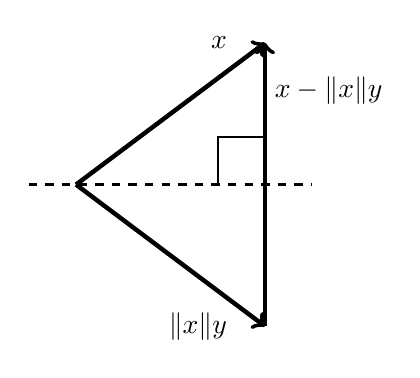
\begin{tikzpicture}[scale=0.6]
    \draw [thick,dashed] (-1,0) -- (5,0);
    \draw [ultra thick,->] (0,0) -- (4,3);
    \draw [ultra thick,->] (0,0) -- (4,-3);
    \draw [ultra thick,->] (4,-3) -- (4,3);
    \draw [thick] (3,0) -- (3,1) -- (4,1);
    \draw (4,2) node [right] {$x-\|x\| y$};
    \draw (3.4,3) node [left] {$x$};
    \draw (3.4,-3) node [left] {$\|x\| y$};
  \end{tikzpicture}
\end{center}
\caption{Construction of a reflector to transform $x$ into $\|x\|y$,
         $\|y\| = 1$.}
\label{fig1}
\end{figure}

Now think about applying a sequence of Householder transformations to
introduce subdiagonal zeros into $A$, just as we used a sequence of Gauss
transformations to introduce subdiagonal zeros in Gaussian elimination.
This leads us to the following algorithm to compute the $QR$
decomposition:
\lstinputlisting{code/hqr1.m}
Note that there are two valid choices of $u_1$ at each step;
we make the choice that avoids cancellation in the obvious version
of the formula.

As with $LU$ factorization, we can re-use the storage of $A$ by recognizing
that the number of nontrivial parameters in the vector $w$ at each step
is the same as the number of zeros produced by that transformation.
This gives us the following:
\lstinputlisting{code/hqr2.m}

If we ever need $Q$ or $Q^T$ explicitly, we can always form it from
the compressed representation.  We can also multiply by $Q$ and $Q^T$
implicitly:
\lstinputlisting{code/applyQ.m}
\lstinputlisting{code/applyQT.m}

\section{Givens rotations}

Householder reflections are one of the standard orthogonal
transformations used in numerical linear algebra.  The other standard
orthogonal transformation is a {\em Givens rotation}:
\[
  G = \begin{bmatrix}
    c & -s \\
    s & c
  \end{bmatrix}.
\]
where $c^2 + s^2 = 1$.  Note that
\[
  G = \begin{bmatrix}
    c & -s \\
    s & c
  \end{bmatrix}
  \begin{bmatrix}
    x \\ y
  \end{bmatrix} =
  \begin{bmatrix}
    cx - sy \\
    sx + cy
  \end{bmatrix}
\]
so if we choose
\begin{align*}
  s &= \frac{-y}{\sqrt{x^2 + y^2}}, &
  c &= \frac{x}{\sqrt{x^2+y^2}}
\end{align*}
then the Givens rotation introduces a zero in the second column.
More generally, we can transform a vector in $\bbR^m$ into a vector
parallel to $e_1$ by a sequence of $m-1$ Givens rotations, where
the first rotation moves the last element to zero, the second rotation
moves the second-to-last element to zero, and so forth.

For some applications, introducing zeros one by one is very
attractive.  In some places, you may see this phrased as a contrast
between algorithms based on Householder reflections and those based on
Givens rotations, but this is not quite right.  Small Householder
reflections can be used to introduce one zero at a time, too.
Still, in the general usage, Givens rotations seem to be the more
popular choice for this sort of local introduction of zeros.

\end{document}
